\documentclass{article}

\usepackage{amsmath}
\usepackage{graphicx}
\usepackage{subcaption}
\usepackage{setspace}

\title{My first document}
\date{2018-09-29}
\author{Marek Dudek}

\setcounter{tocdepth}{1}

\begin{document}

    \pagenumbering{gobble}
    \maketitle

    \newpage
    \doublespacing
    \tableofcontents
    \singlespacing

    \newpage
    \pagenumbering{arabic}

    \section{Section}
    Hello World!
    \subsection{Subsection}
    Structuring a document is easy!
    \subsubsection{Subsubsection}
    This is sub-subsection.
    \paragraph{Paragraph}
    This is a paragraph.
    \subparagraph{Subparagraph}
    This is a subparagraph.

    \section{Another section}

    \section{Math}

	    \begin{equation}
		f(x) = x^2
	    \end{equation}
	    \begin{equation*}
		f(x) = x^2
	    \end{equation*}

        This formula $f(x) = x^2$ is an example of embedded formula.

    \begin{align*}
 	1 + 2 &= 3\\
 	1 &= 3 - 2
    \end{align*}

    \begin{align*}
 	f(x) &= x^2\\
	g(x) &= \frac{1}{x}\\
	F(x) &= \int^a_b \frac{1}{3}x^3\\
	G(x) &= \frac{1}{\sqrt{x}}
    \end{align*}

    \begin{equation*}
	    \begin{matrix}
		1 & 0\\
		0 & 1
	    \end{matrix}
    \end{equation*}

    \begin{equation*}
	    \begin{bmatrix}
		1 & 0\\
		0 & 1
	    \end{bmatrix}
    \end{equation*}

    \begin{equation*}
	[
	\begin{matrix}
	    1 & 0\\
	    0 & 1
	\end{matrix}
	]
    \end{equation*}

    \begin{equation*}
	\left[
	\begin{matrix}
	    1 & 0\\
	    0 & 1
	\end{matrix}
	\right]
    \end{equation*}

    \begin{equation*}
	\left(\frac{1}{\sqrt{x}}\right)
    \end{equation*}

    This is $\lambda$!

    \newpage

    \section{Pictures}

    \begin{figure}[h!]
	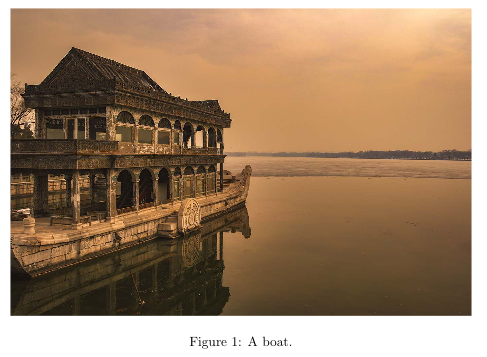
\includegraphics[width=\linewidth]{images/boat.png}
	\caption{A boat.}
	\label{fig:boat1}
    \end{figure}

    Figure \ref{fig:boat1} shows a boat.

    \begin{figure}[h!]
	\centering
	\begin{subfigure}[b]{0.4\linewidth}
		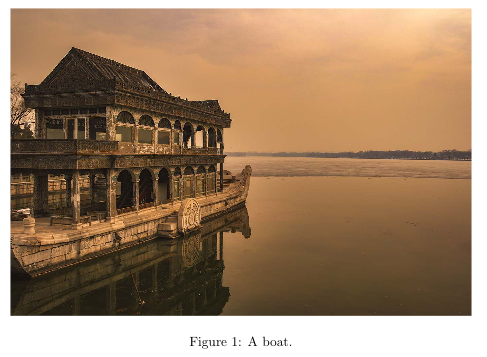
\includegraphics[width=\linewidth]{images/boat.png}
		\caption{A boat.}
	\end{subfigure}
	\begin{subfigure}[b]{0.4\linewidth}
		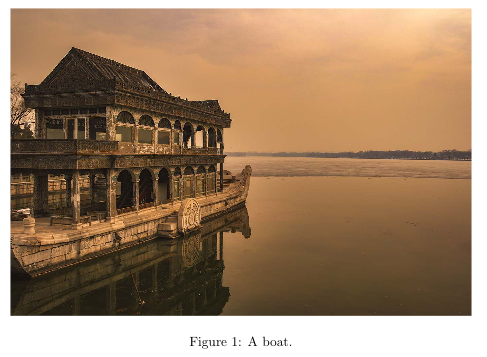
\includegraphics[width=\linewidth]{images/boat.png}
		\caption{Another boat.}
	\end{subfigure}
	\caption{The same boat two times.}
	\label{fig:twoboats}
    \end{figure}

    \newpage

    \section{Tables}

    \begin{table}[h!]
	\caption{Dummy table}
    \end{table}

    \newpage

    \section{Using BibTeX}

    Random citation \cite{DUMMY:1} embedded in text.
    
    \begin{appendix}
	\listoffigures
	\listoftables
    \end{appendix}

    \bibliography{dummy}
    \bibliographystyle{ieeetr}

\end{document}
